\documentclass[12pt,letterpaper]{article}
\usepackage[utf8]{inputenc}
\usepackage[spanish]{babel}
\usepackage{graphicx}
\usepackage[left=2cm,right=2cm,top=2cm,bottom=2cm]{geometry}
\usepackage{graphicx} % figuras
% \usepackage{subfigure} % subfiguras
\usepackage{float} % para usar [H]
\usepackage{amsmath}
%\usepackage{txfonts}
\usepackage{stackrel} 
\usepackage{multirow}
\usepackage{enumerate} % enumerados
\renewcommand{\labelitemi}{$-$}
\renewcommand{\labelitemii}{$\cdot$}


% \author{}
% \title{Caratula}
\begin{document}

% Fancy Header and Footer
% \usepackage{fancyhdr}
% \pagestyle{fancy}
% \cfoot{}
% \rfoot{\thepage}
%

% \usepackage[hidelinks]{hyperref} % CREA HYPERVINCULOS EN INDICE

% \author{}
\title{Caratula}

\begin{titlepage}
\begin{center}
\large{UNIVERSIDAD PRIVADA DE TACNA}\\
\vspace*{-0.025in}
\begin{figure}[htb]
\begin{center}

\includegraphics[width=8cm]{./Imagenes/logo}
\end{center}
\end{figure}
\vspace*{0.15in}
INGENIERÍA DE SISTEMAS  \\

\vspace*{0.5in}
\begin{large}
TITULO:\\
\end{large}

\vspace*{0.1in}
\begin{Large}
\textbf{Informe de laboratorio 01 - Gestion y planeamiento de pruebas} \\
\end{Large}

\vspace*{0.3in}
\begin{Large}
\textbf{CURSO:} \\
\end{Large}

\vspace*{0.1in}
\begin{large}
Calidad y Pruebas de Software\\
\end{large}

\vspace*{0.3in}
\begin{Large}
\textbf{DOCENTE(ING):} \\
\end{Large}

\vspace*{0.1in}
\begin{large}
 Patrick Cuadros Quiroga\\
\end{large}

\vspace*{0.2in}
\vspace*{0.1in}
\begin{large}
Integrante: \\
\begin{flushleft}
Percy Taquila Carazas\hfill	(2018061088) \\
\end{flushleft}
\end{large}
\end{center}

\end{titlepage}

\tableofcontents % INDICE
\thispagestyle{empty} % INDICE SIN NUMERO
\newpage
\setcounter{page}{1} % REINICIAR CONTADOR DE PAGINAS DESPUES DEL INDICE


\section{Objetivos} 
\begin{itemize}
\item crear y administrar planes de prueba, conjuntos de pruebas y casos de prueba.
\end{itemize}



\section{Requerimientos} 

\begin{itemize}
\item Esta práctica de laboratorio requiere que complete las tareas 1 y 2 de las instrucciones de requisitos previos (Azure DevOps)

\end{itemize}



\section{Desarrollo}

\textbf{Ejercicio 1: Gestión de casos, conjuntos y planes de prueba}\\
En este ejercicio, aprenderá a crear y administrar planes de prueba, conjuntos de pruebas y casos de prueba.\\

\textbf{Tarea 1: Comprensión de casos, conjuntos y planes de prueba}

1. Navegue hasta el proyecto de su equipo en Azure DevOps.\\

2. Seleccione Test Plans para navegar hasta Test Hub . El centro de pruebas proporciona un lugar central para toda la planificación, ejecución y análisis de pruebas.

\begin{center}
		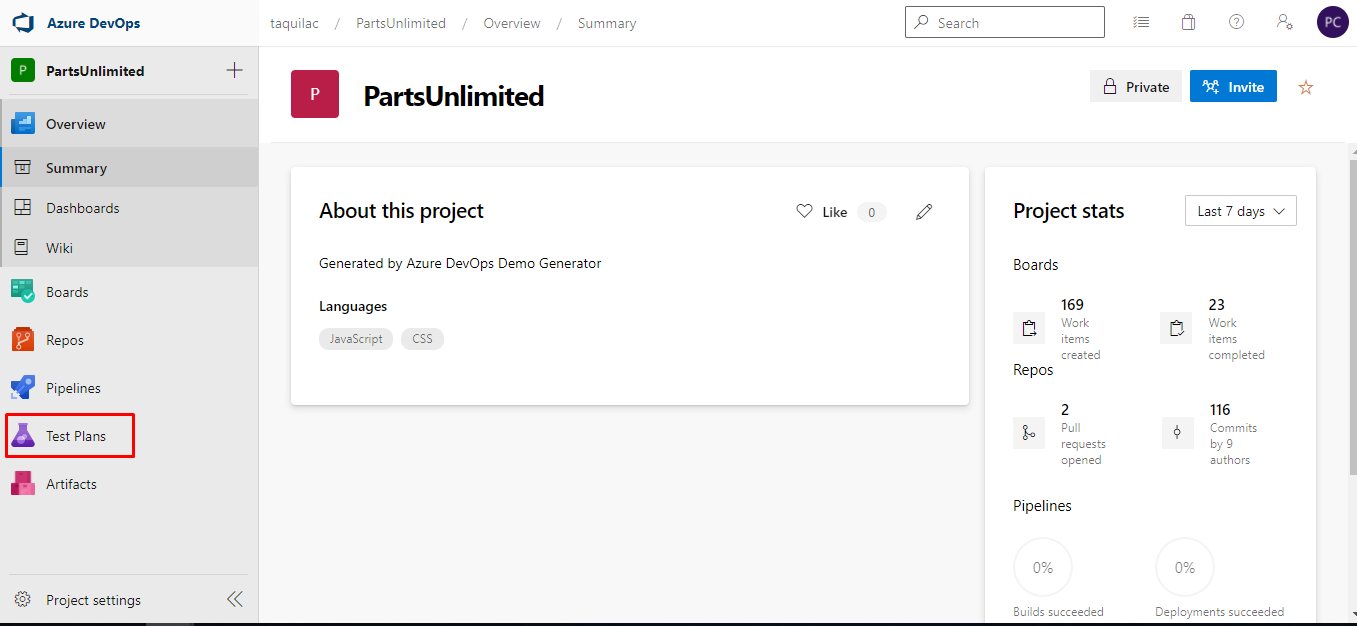
\includegraphics[width=15cm]{./Imagenes/1} 
\end{center}

3. En general, cada hito importante de un proyecto debe tener su propio  test plan. Dentro de cada plan de prueba hay test suites, que son colecciones de test cases(y, opcionalmente, otros conjuntos de pruebas) diseñados para validar un elemento de trabajo, como la implementación de una función o la corrección de errores. Cada caso de prueba está diseñado para confirmar un comportamiento específico y puede pertenecer a uno o más conjuntos de pruebas. El proyecto Parts Unlimited tiene un plan de prueba, que está bajo el Parts Unlimited team y se llama Parts Unlimited\_TestPlan1 . Seleccione el plan de prueba Parts Unlimited\_TestPlan1.

\begin{center}
		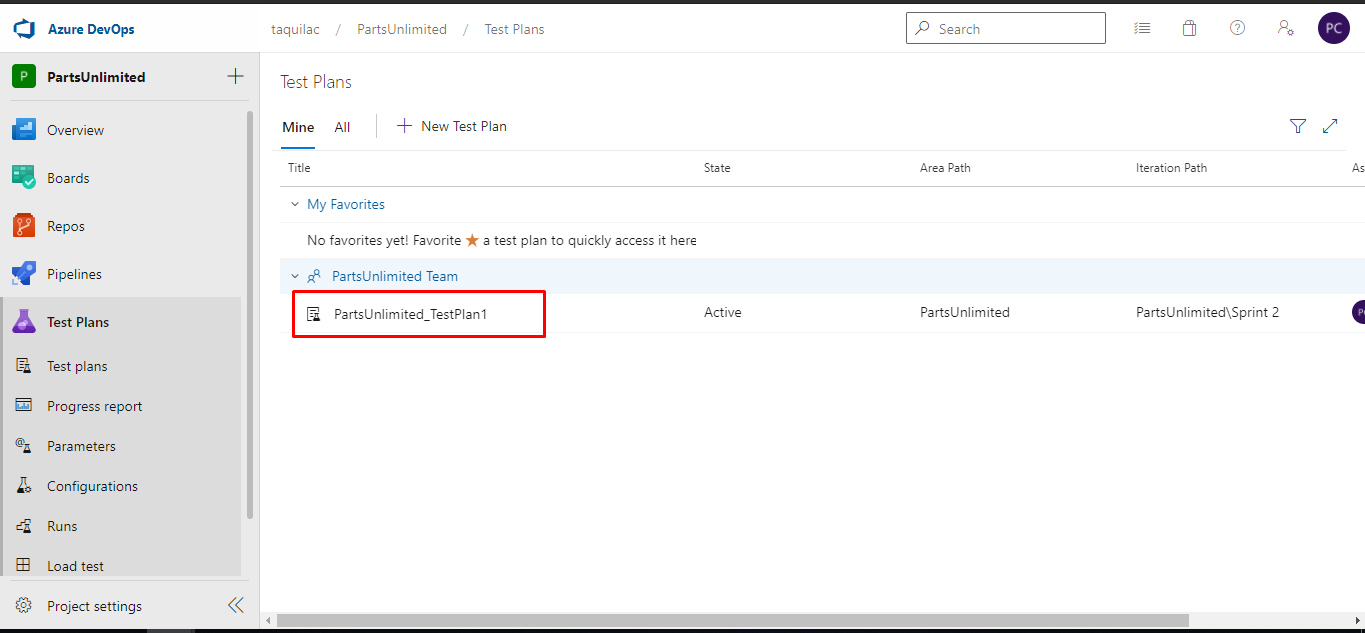
\includegraphics[width=15cm]{./Imagenes/2} 
\end{center}

4. Seleccione el conjunto de pruebas para la historia As a customer, I would like to store my credit card details securely. Este conjunto de pruebas se centra en ese elemento de trabajo, que resulta ser una función. Tenga en cuenta que los números de los elementos de trabajo variarán cada vez que genere datos de demostración para un laboratorio.

\begin{center}
		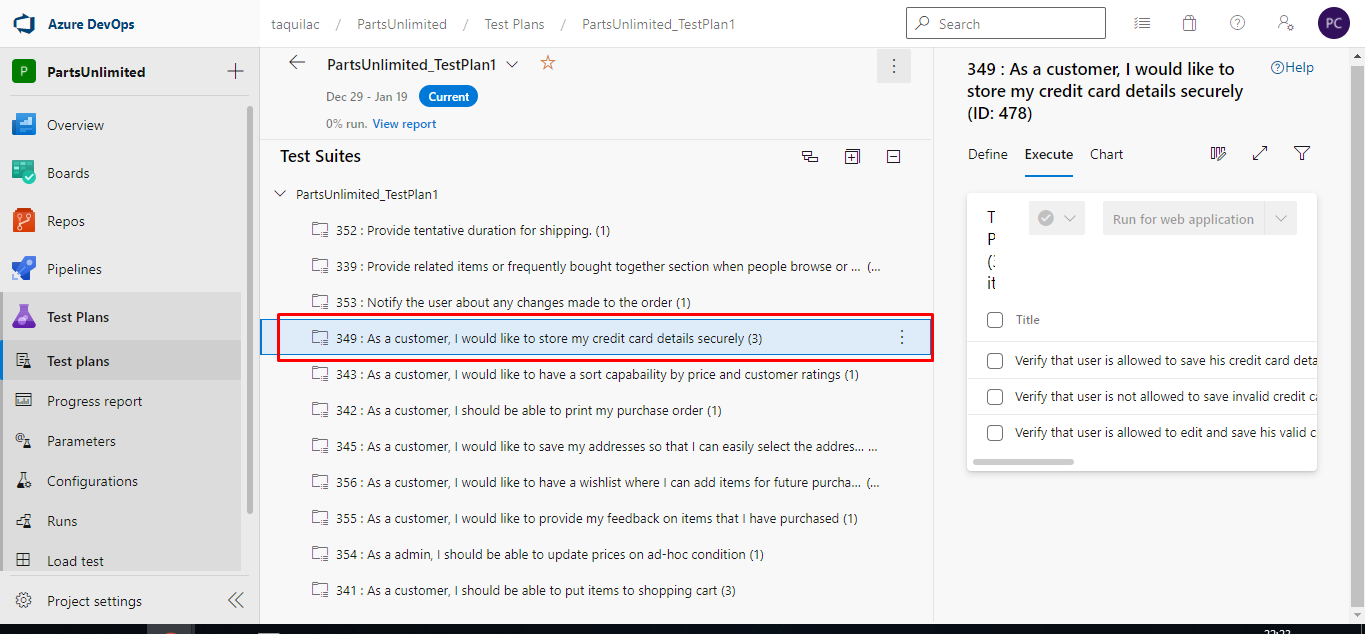
\includegraphics[width=15cm]{./Imagenes/3} 
\end{center}

5. En el lado derecho, puede ver que este conjunto de pruebas tiene tres casos de prueba diseñados para confirmar el comportamiento esperado de la implementación de la función. Haga doble clic en Verify that user is allowed to save his credit card detail

\begin{center}
		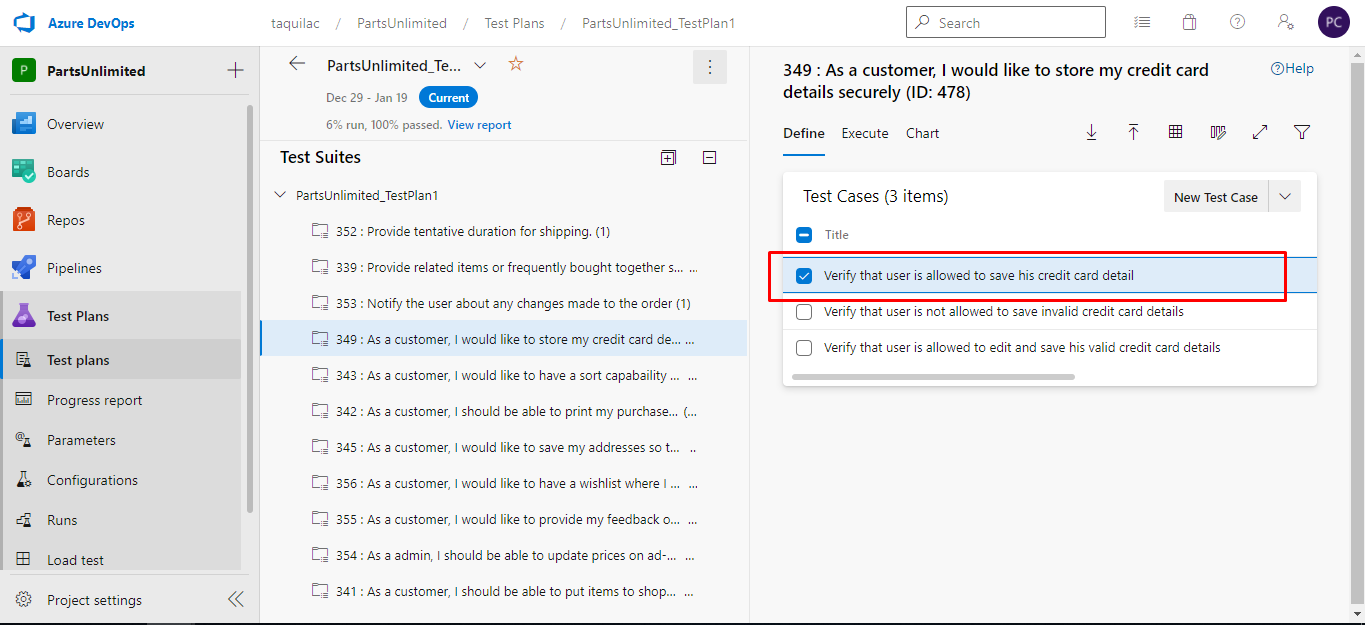
\includegraphics[width=15cm]{./Imagenes/4} 
\end{center}

6. Este cuadro de diálogo proporciona toda la información que necesita sobre este caso de prueba. Busque el panelRelated Work y tenga en cuenta que este caso de prueba está vinculado a la suite a la que pertenece. Haga clic en el elemento de trabajo para navegar hasta él.

\begin{center}
		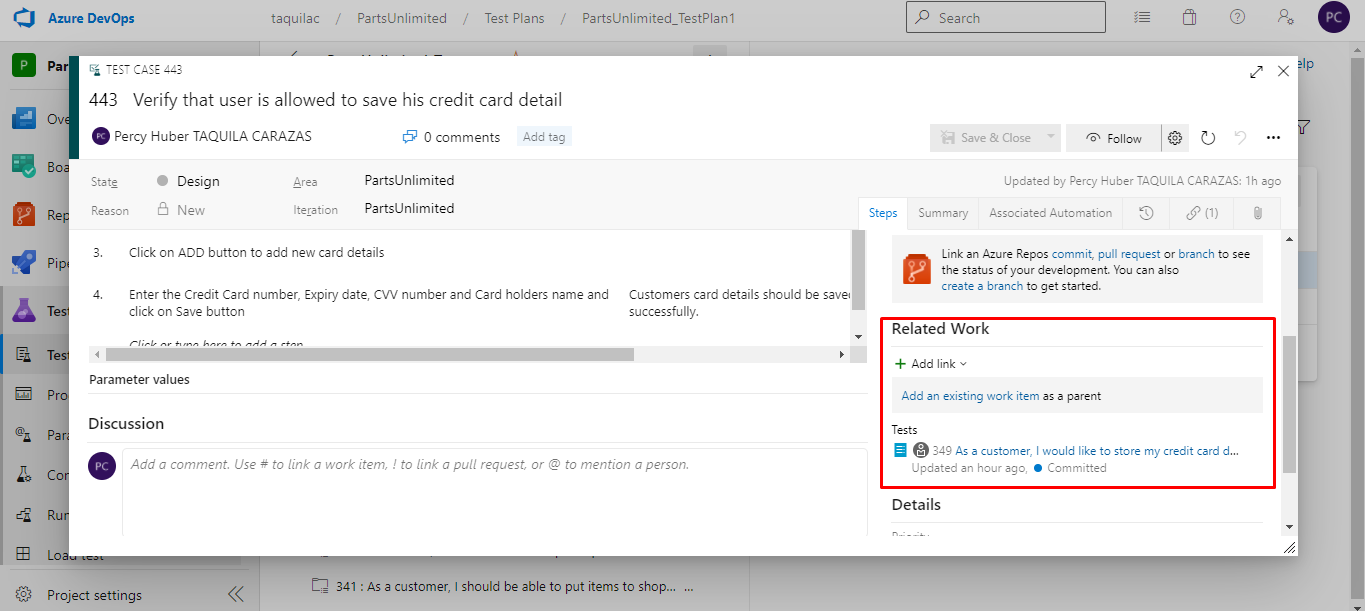
\includegraphics[width=15cm]{./Imagenes/5} 
\end{center}

7. En el conjunto de pruebas, podemos ver todos los elementos de trabajo vinculados, que resultan ser los casos de prueba.

\begin{center}
		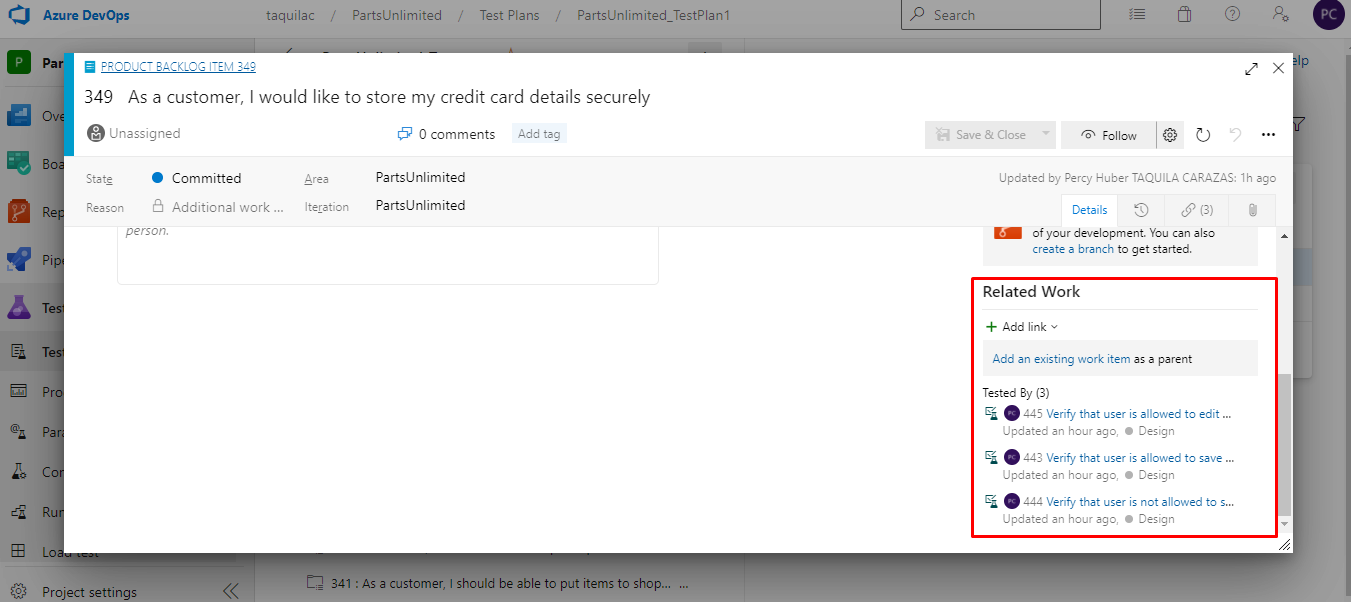
\includegraphics[width=15cm]{./Imagenes/6} 
\end{center}

8. Sin embargo, aún no está asociado con la función para la que está diseñado para probar, que podemos vincular ahora. Haga clic en Add link | Existing item.

\begin{center}
		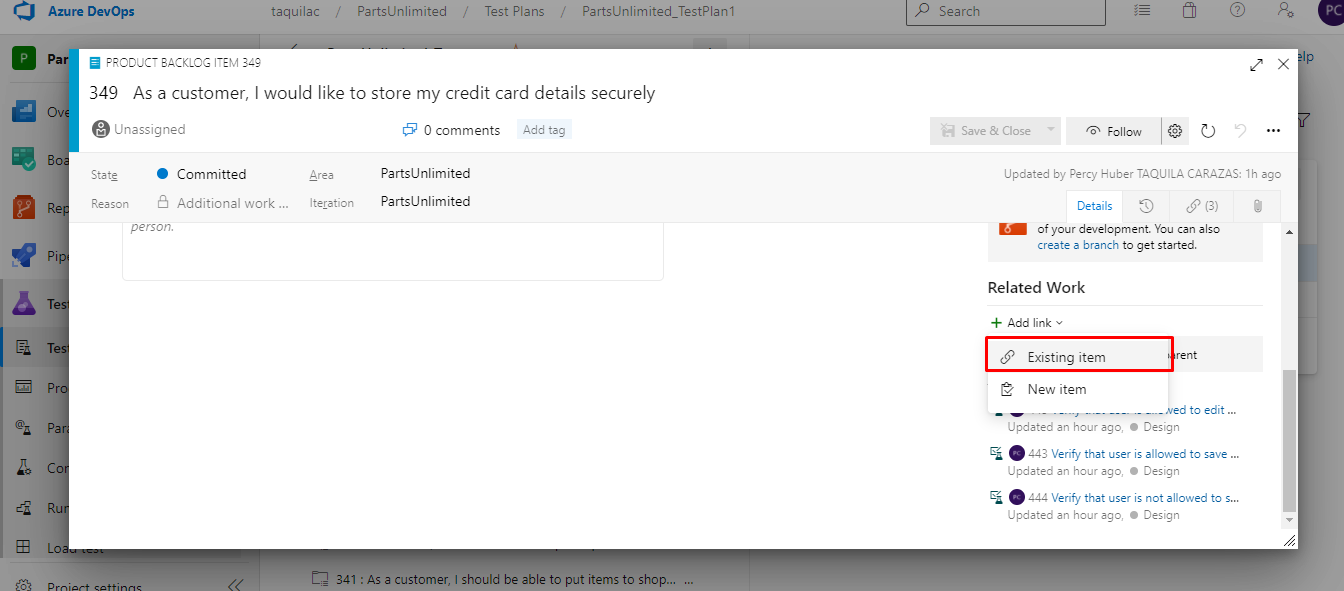
\includegraphics[width=15cm]{./Imagenes/7} 
\end{center}

9. Establezca el Link type en Parent  y busque “credit card”.

\begin{center}
		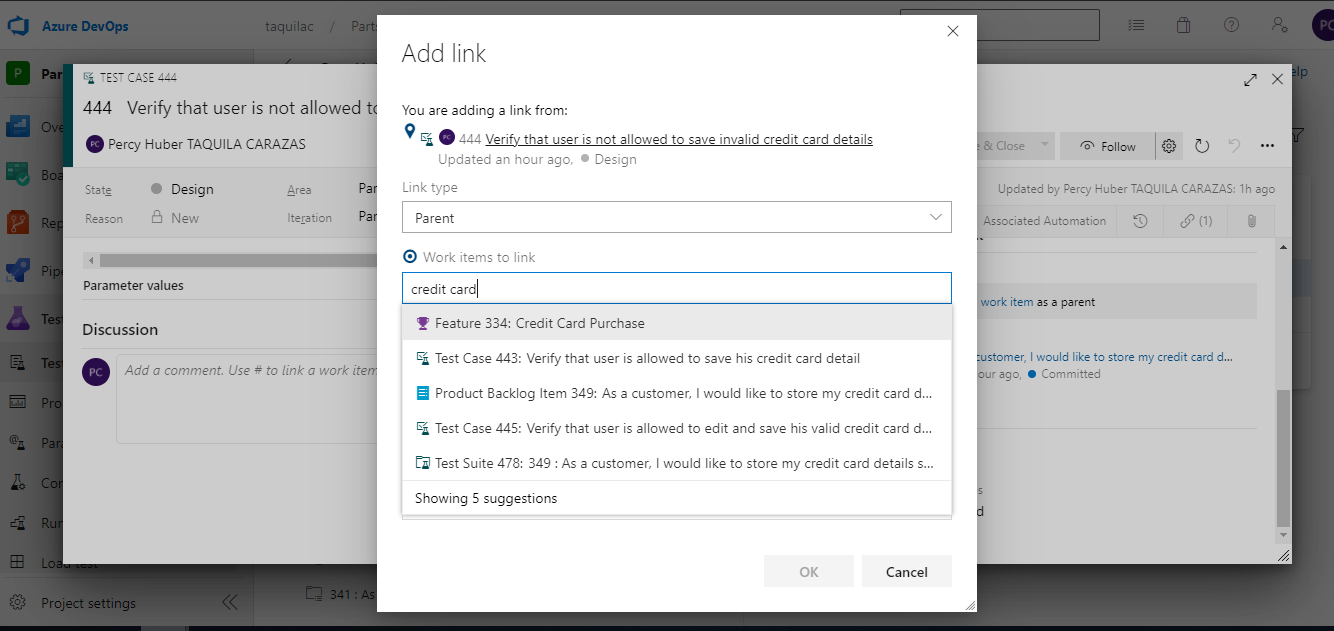
\includegraphics[width=15cm]{./Imagenes/8} 
\end{center}

10. Feature Credit Card Purchase.

\begin{center}
		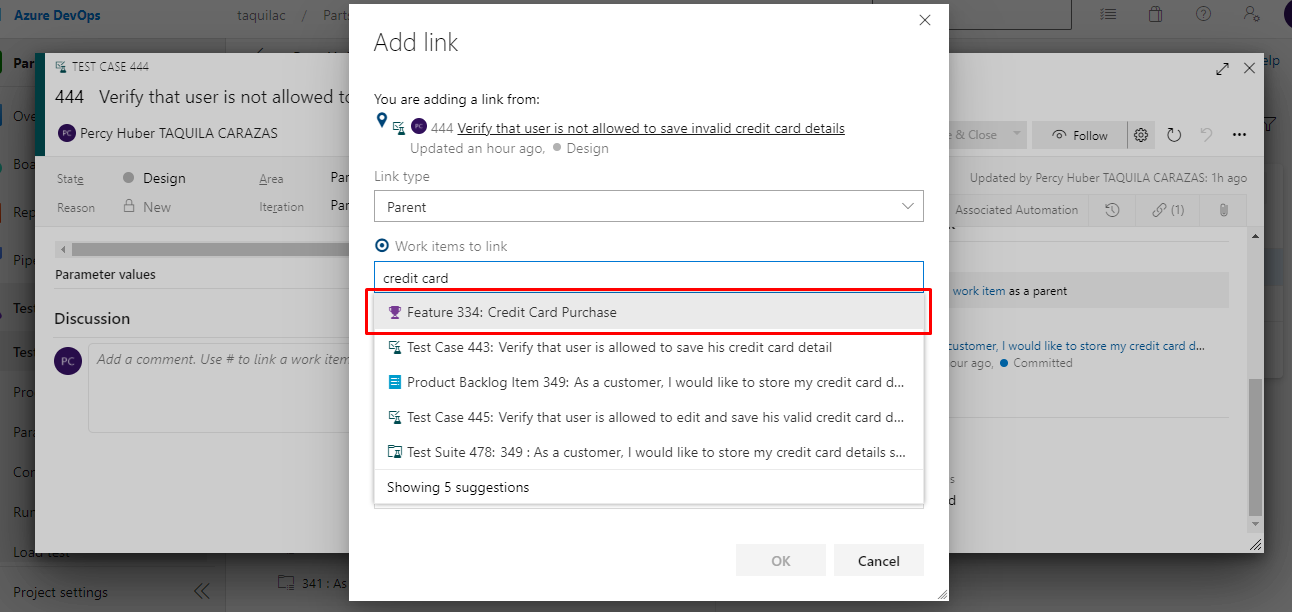
\includegraphics[width=15cm]{./Imagenes/9} 
\end{center}

11. Click OK.

\begin{center}
		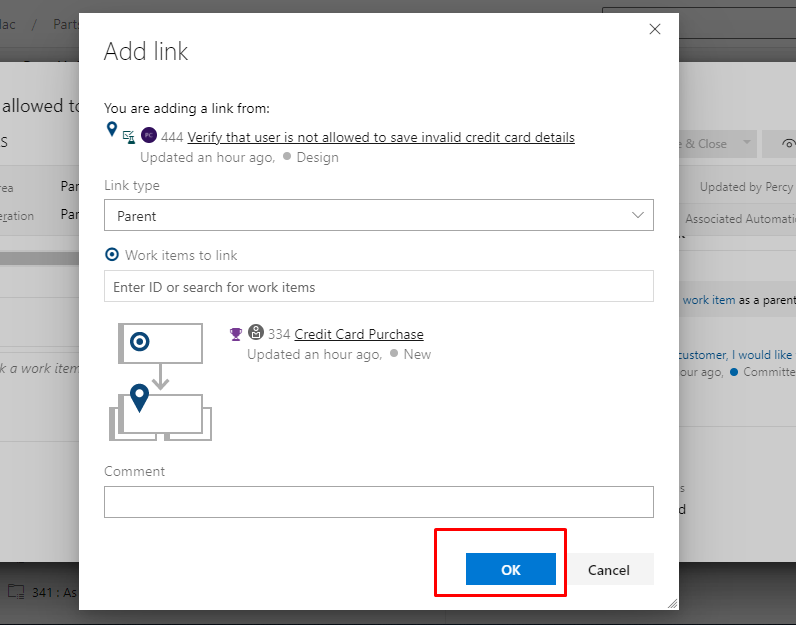
\includegraphics[width=12cm]{./Imagenes/10} 
\end{center}

12. La función principal ahora está asociada con la suite que la prueba y cualquiera puede navegar entre ellos para ver su relación en relación con los otros elementos de trabajo involucrados.

\begin{center}
		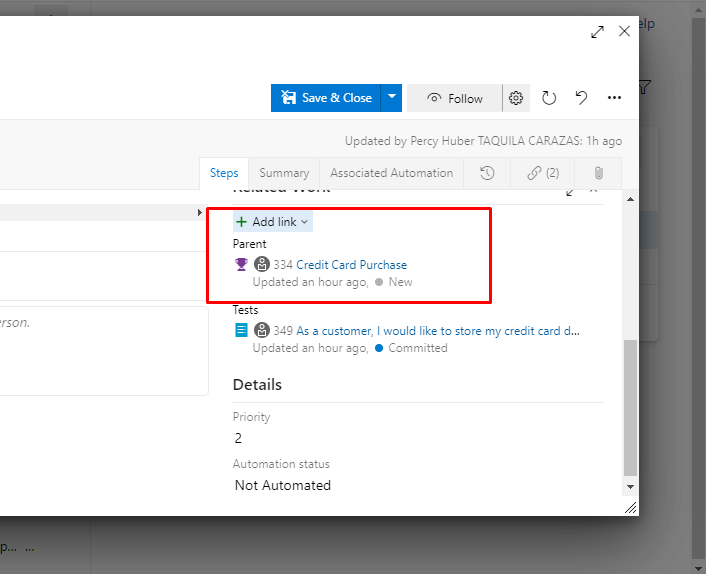
\includegraphics[width=12cm]{./Imagenes/11} 
\end{center}

13. Click Save \& Close.

\begin{center}
		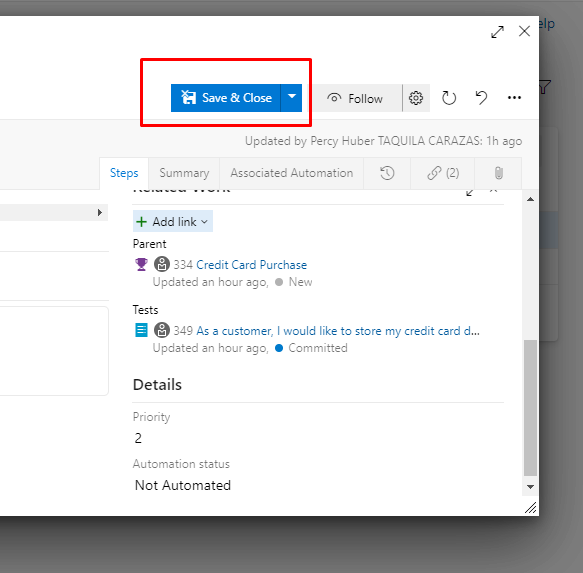
\includegraphics[width=15cm]{./Imagenes/12} 
\end{center}

14. Descarte el cuadro de diálogo del caso de prueba original.\\

\textbf{Tarea 2: Gestión de pruebas}\\

1. A veces, se debe ejecutar un conjunto de casos de prueba en un orden específico para maximizar la eficiencia. Haga clic en Order tests para especificar el orden en que se deben ejecutar estos casos de prueba.\\

2. Si bien estos casos de prueba se pueden ejecutar por separado para confirmar el comportamiento, probablemente tenga más sentido ejecutar primero el caso de prueba que rechaza las tarjetas no válidas. Luego, el probador puede confirmar que se puede guardar una tarjeta válida, seguido del caso de prueba para editar una tarjeta guardada. Arrastre y suelte el segundo caso de prueba sobre el primero y haga clic en Done.

\begin{center}
		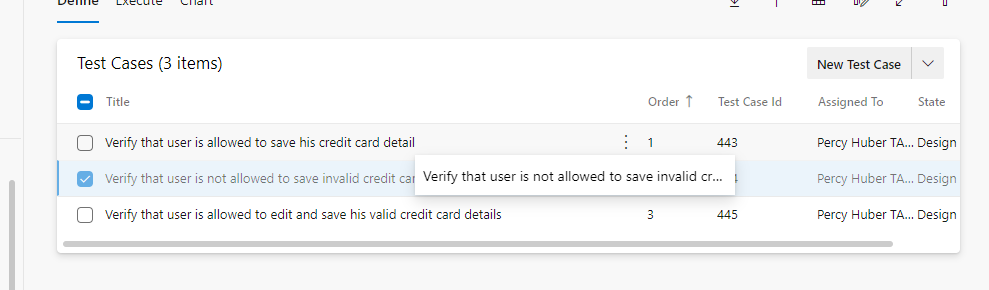
\includegraphics[width=15cm]{./Imagenes/13} 
\end{center}

3. Ahora puede ver que el order se ha actualizado y que la lista ahora está ordenada por él.

\begin{center}
		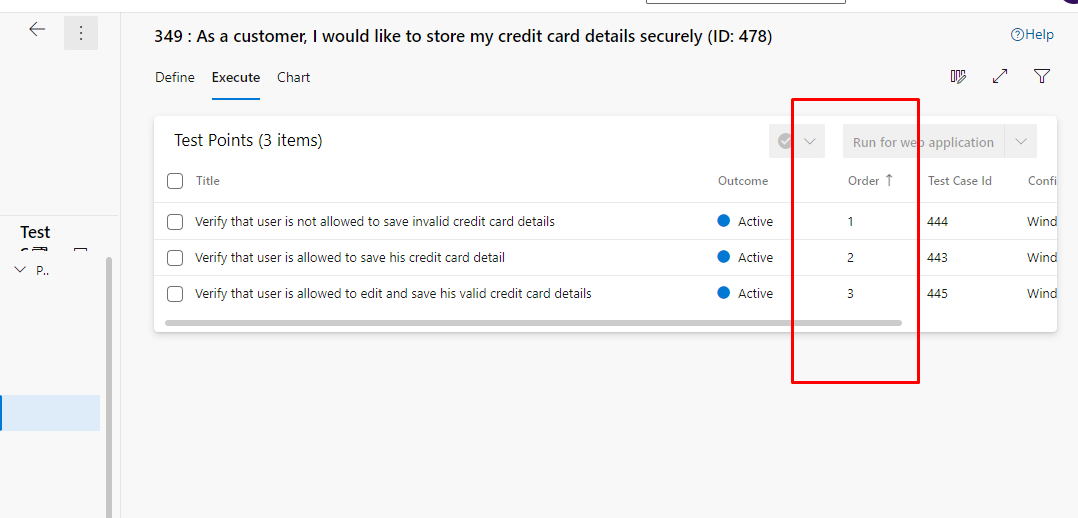
\includegraphics[width=15cm]{./Imagenes/14} 
\end{center}

4. Otro aspecto importante de las pruebas tiene que ver con el entorno en el que se ejecuta cada prueba. Para esta aplicación web, el navegador y el sistema operativo son consideraciones clave. En este momento, todas las pruebas solo usan una configuración: Windows 10.

\begin{center}
		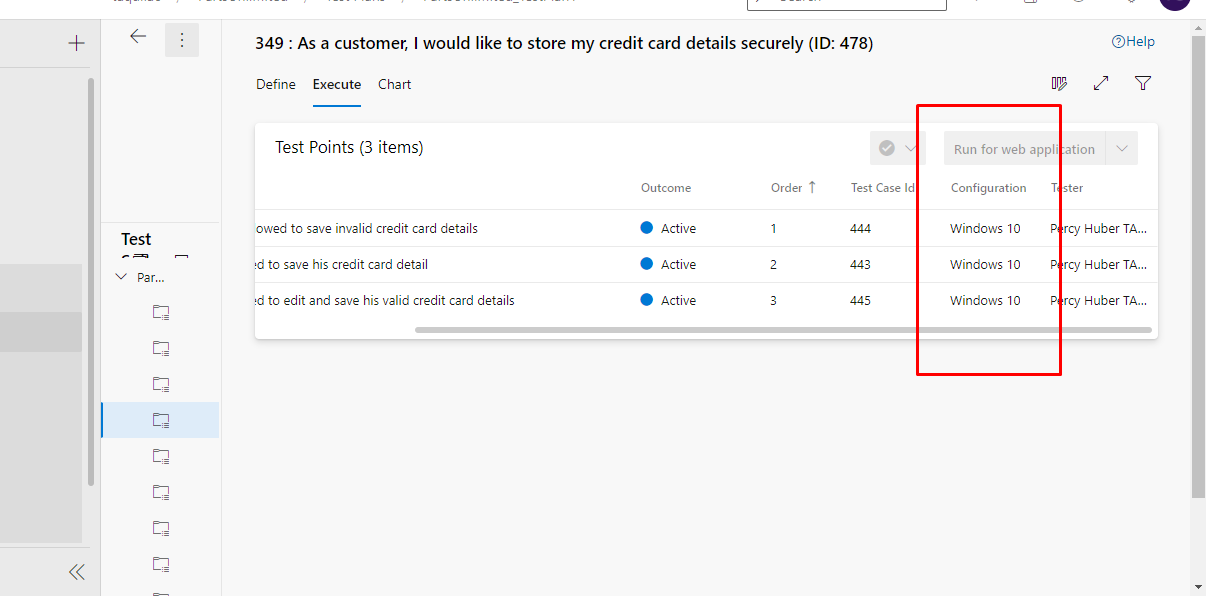
\includegraphics[width=15cm]{./Imagenes/15} 
\end{center}

5. Seleccione la pestaña Configurations.

\begin{center}
		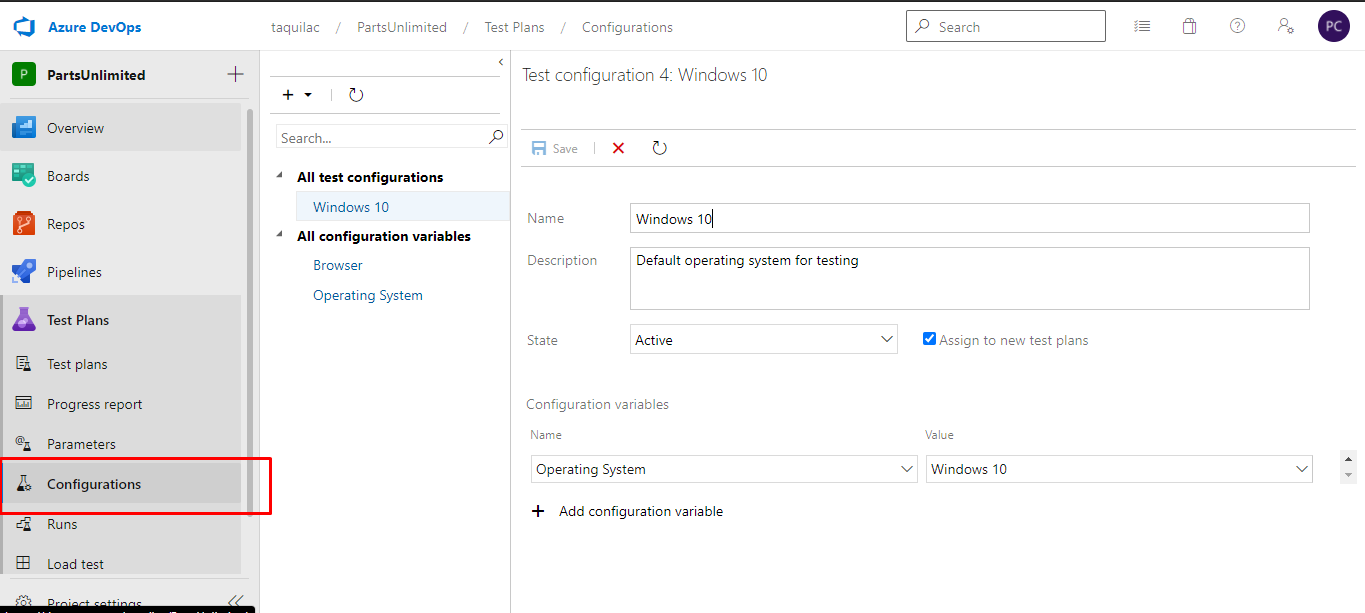
\includegraphics[width=15cm]{./Imagenes/16} 
\end{center}

6. Tenga en cuenta que hay una configuración existente para Windows 10.  Cada configuración de prueba incluye un nombre y una descripción, así como un conjunto de variables de configuración personalizables . Este proyecto tiene una variable de configuración establecida para el sistema operativo . Puede agregar fácilmente más y / o editar las entradas disponibles para cada uno. Haga clic en Agregar variable de configuración.

\begin{center}
		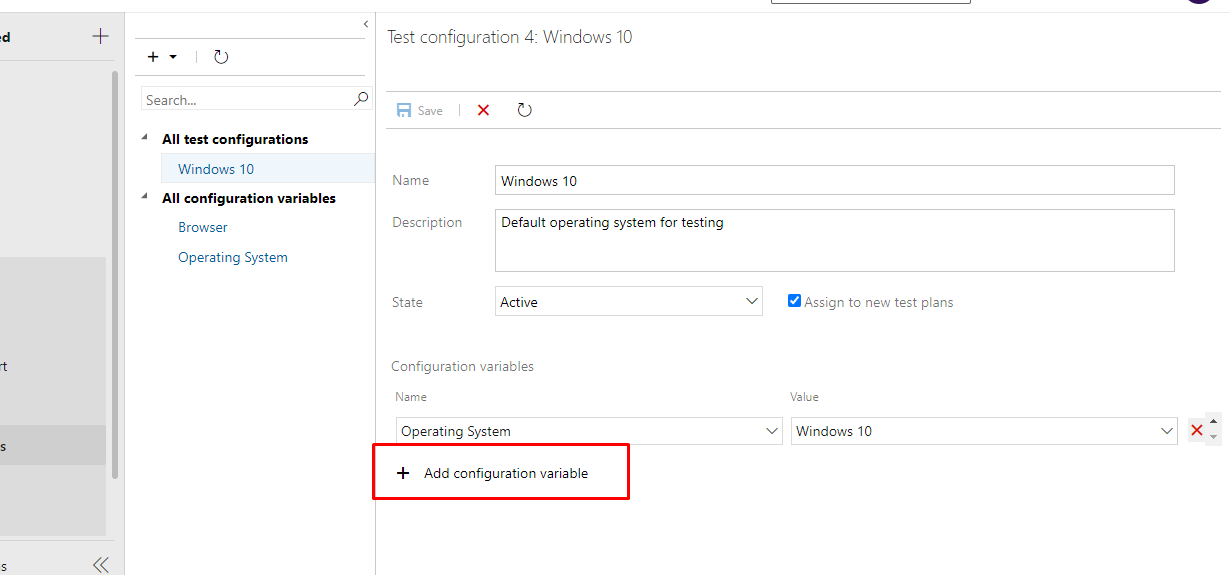
\includegraphics[width=15cm]{./Imagenes/17} 
\end{center}

7. Seleccione la variable del Browser y configúrela en Microsoft Edge.

\begin{center}
		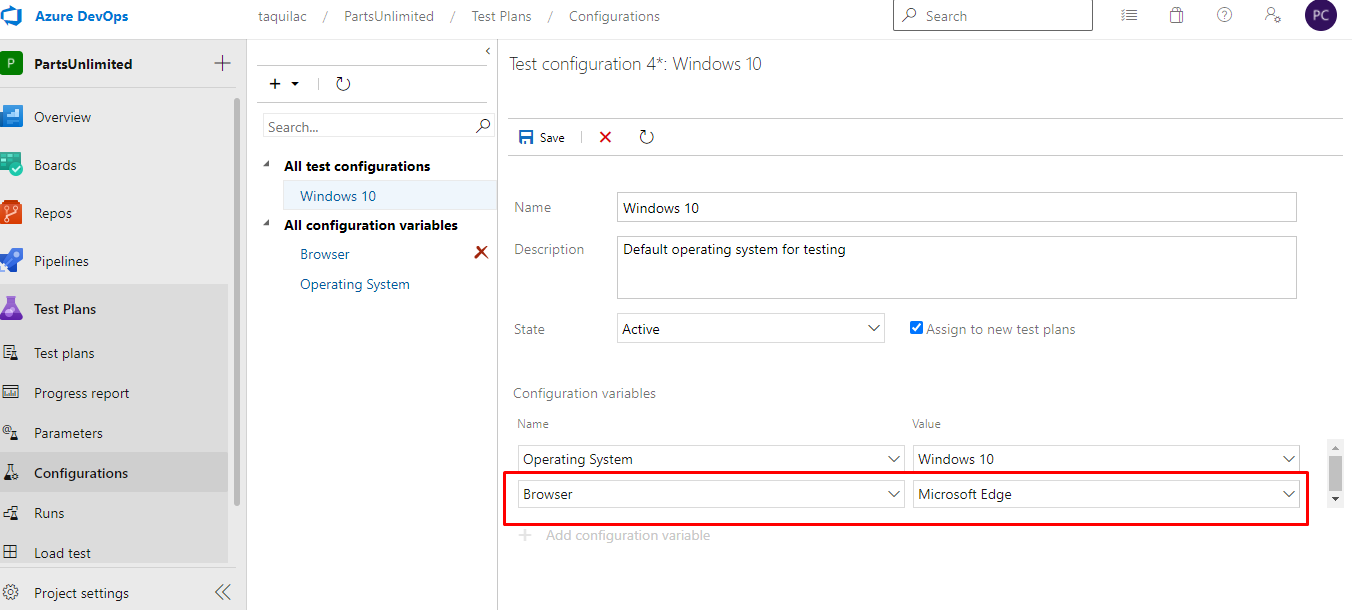
\includegraphics[width=15cm]{./Imagenes/18} 
\end{center}

8. Haga clic en Guardar para Save la configuración.

\begin{center}
		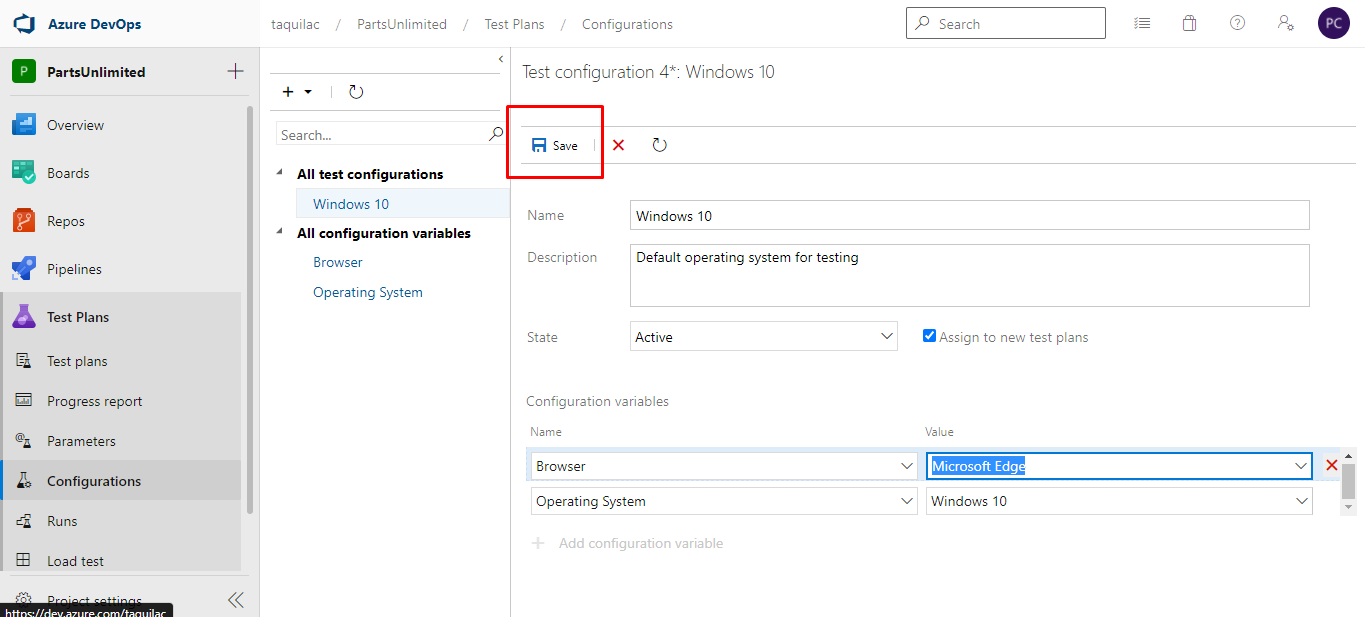
\includegraphics[width=15cm]{./Imagenes/19} 
\end{center}

9. Ahora supongamos que el equipo de prueba ha adquirido un iPhone X y quiere agregarlo a la matriz de prueba. Es realmente fácil registrar este entorno como una nueva configuración para que los casos de prueba puedan especificarlo. Sin embargo, antes de agregarlo, necesitaremos una opción de Operating System para iOS 10 . Haga clic en la variable de configuración del Operating System.

\begin{center}
		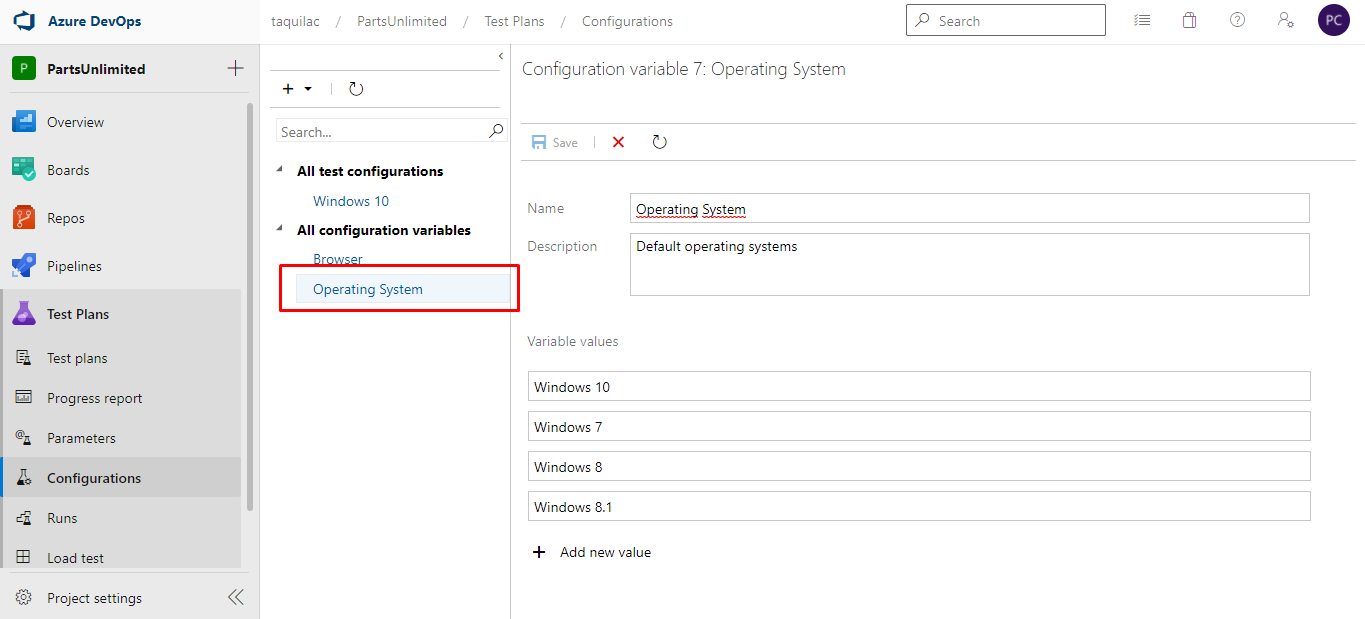
\includegraphics[width=15cm]{./Imagenes/20} 
\end{center}

10. Haga clic en Add new value y agregue una entrada para iOS 12.

\begin{center}
		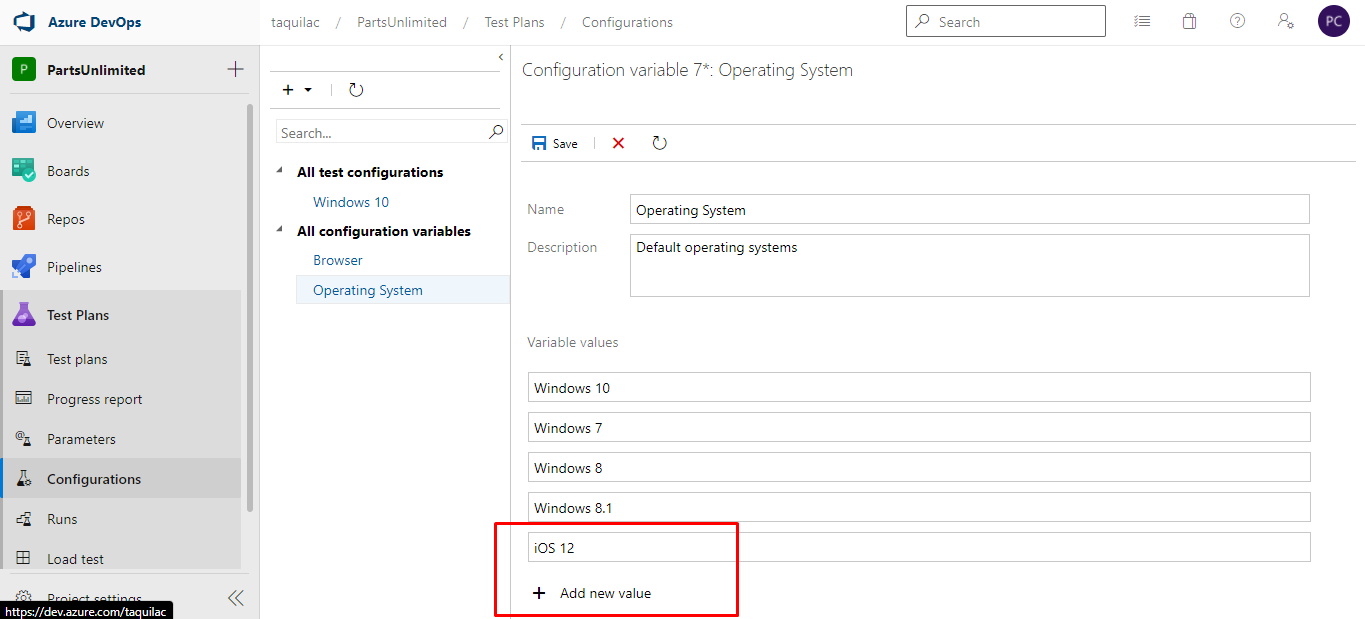
\includegraphics[width=15cm]{./Imagenes/21} 
\end{center}

11. Clic Save

\begin{center}
		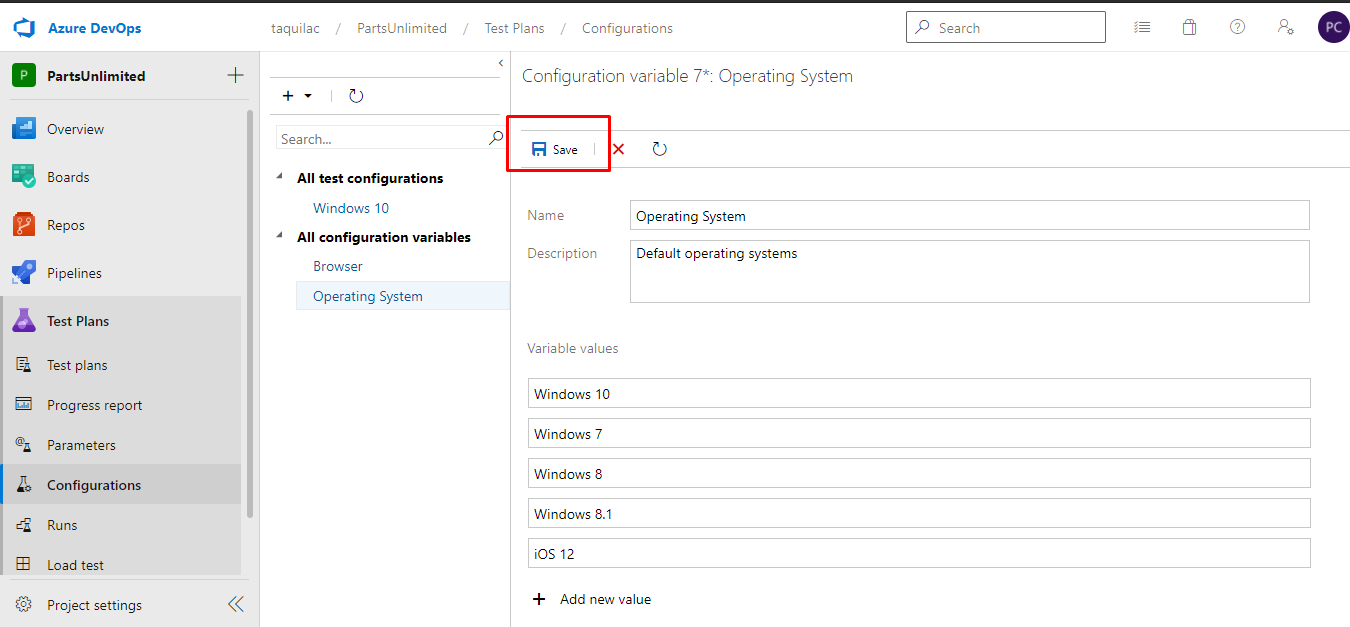
\includegraphics[width=15cm]{./Imagenes/22} 
\end{center}

12. Ahora tenemos todo lo que necesitamos para agregar el iPhone X. Haga clic en el menú desplegable Agregar y seleccione New test configuration.

\begin{center}
		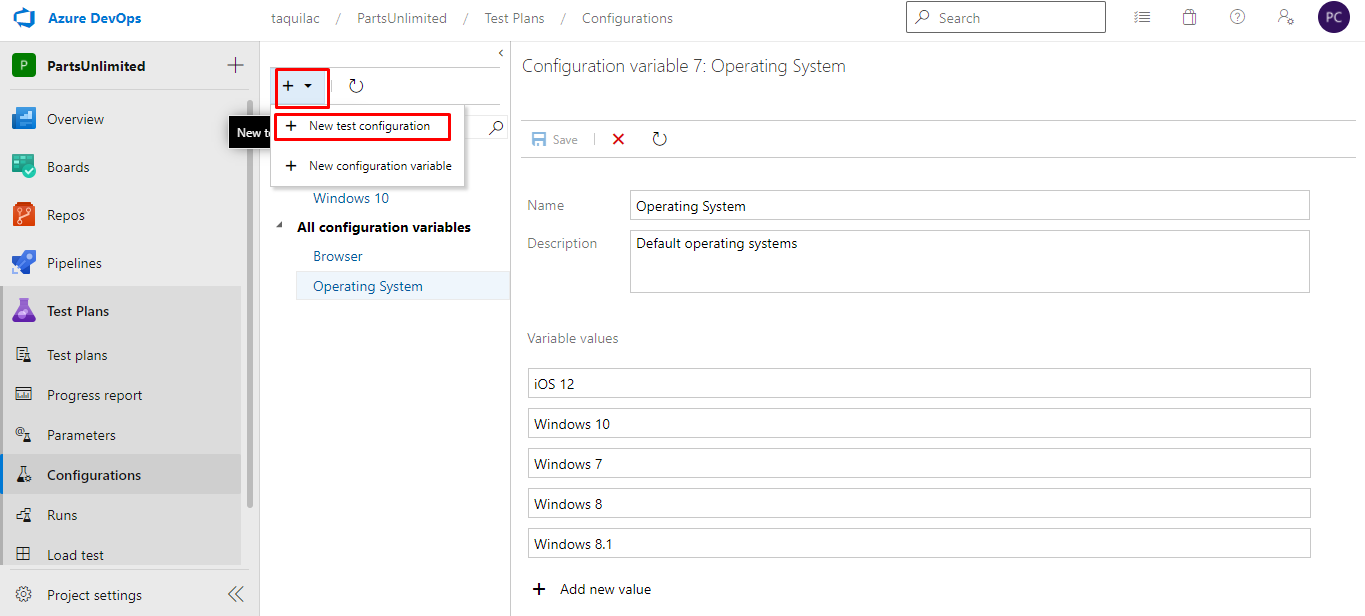
\includegraphics[width=15cm]{./Imagenes/23} 
\end{center}

13. Establezca el nombre en "iPhone X" .

\begin{center}
		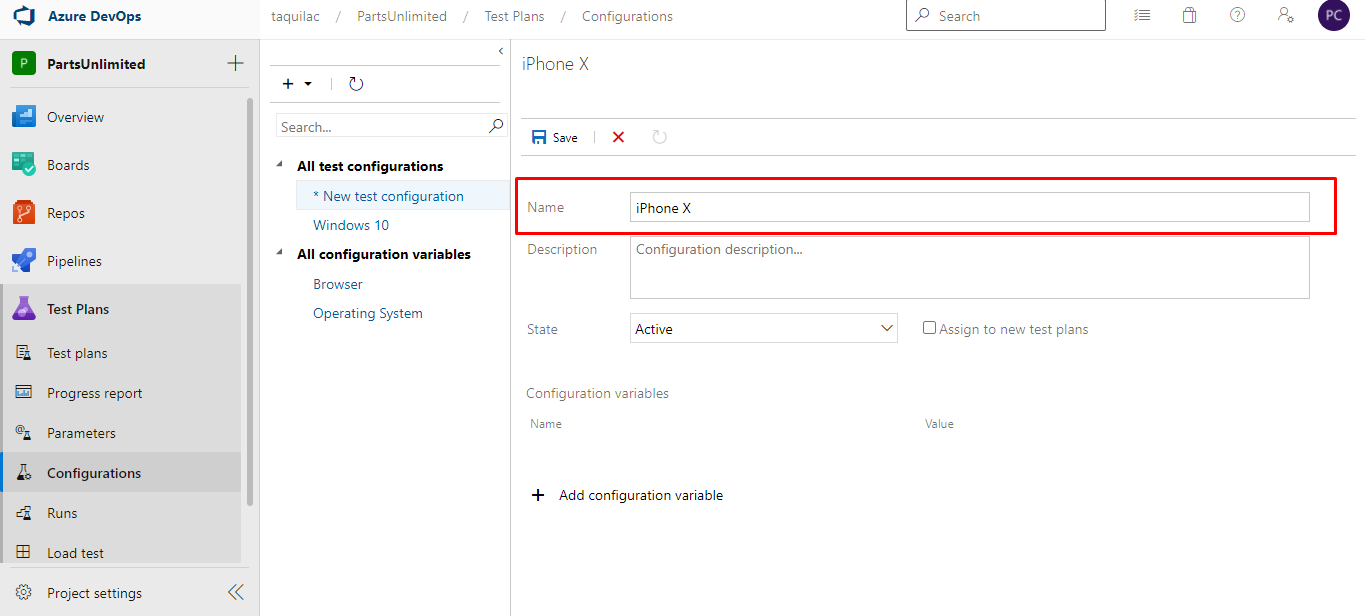
\includegraphics[width=15cm]{./Imagenes/24} 
\end{center}

14. Haga clic en Add Configuration variable dos veces y configure el navegador en Safari y el sistema operativo en iOS 12.

\begin{center}
		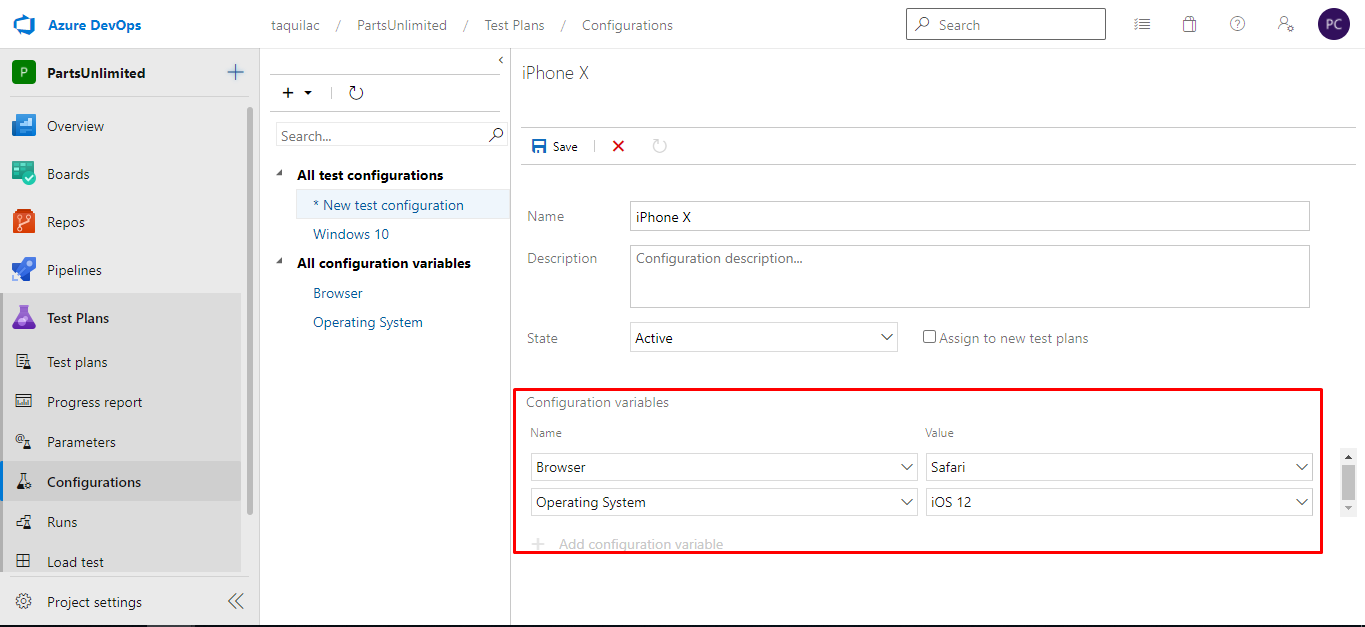
\includegraphics[width=15cm]{./Imagenes/25} 
\end{center}

15. Haga clic en Guardar para Save la nueva configuración.

\begin{center}
		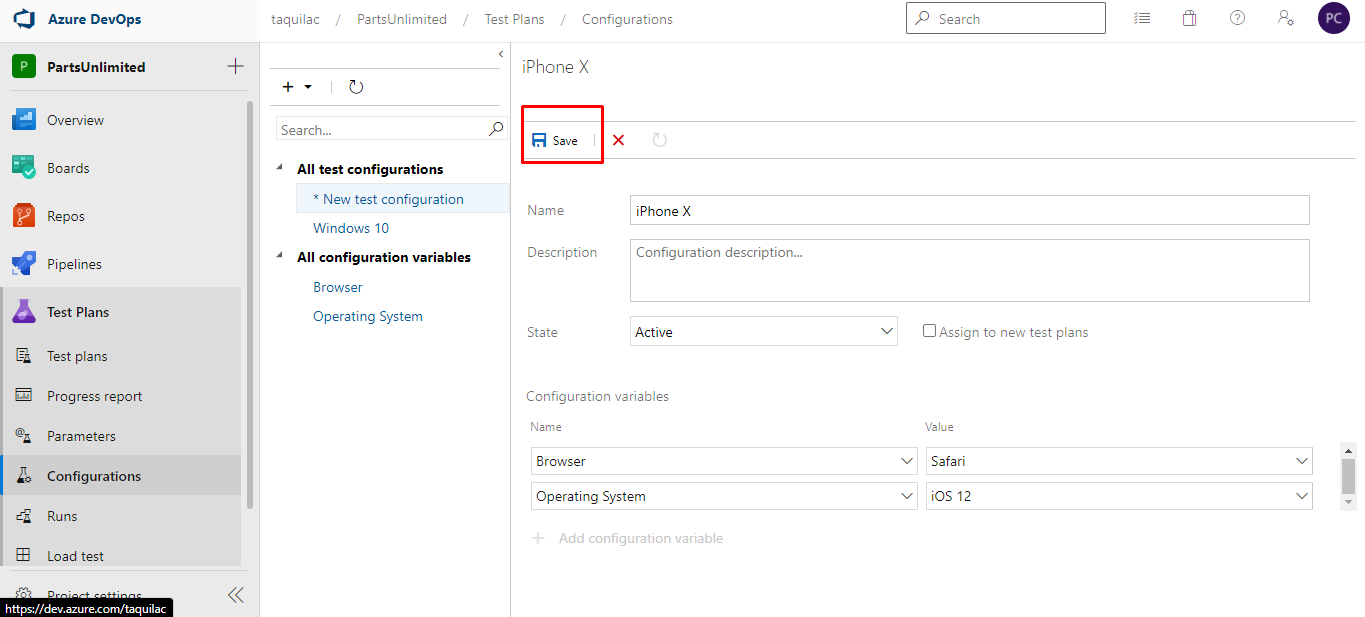
\includegraphics[width=15cm]{./Imagenes/26} 
\end{center}

16. Regrese a la pestaña Test Plans

\begin{center}
		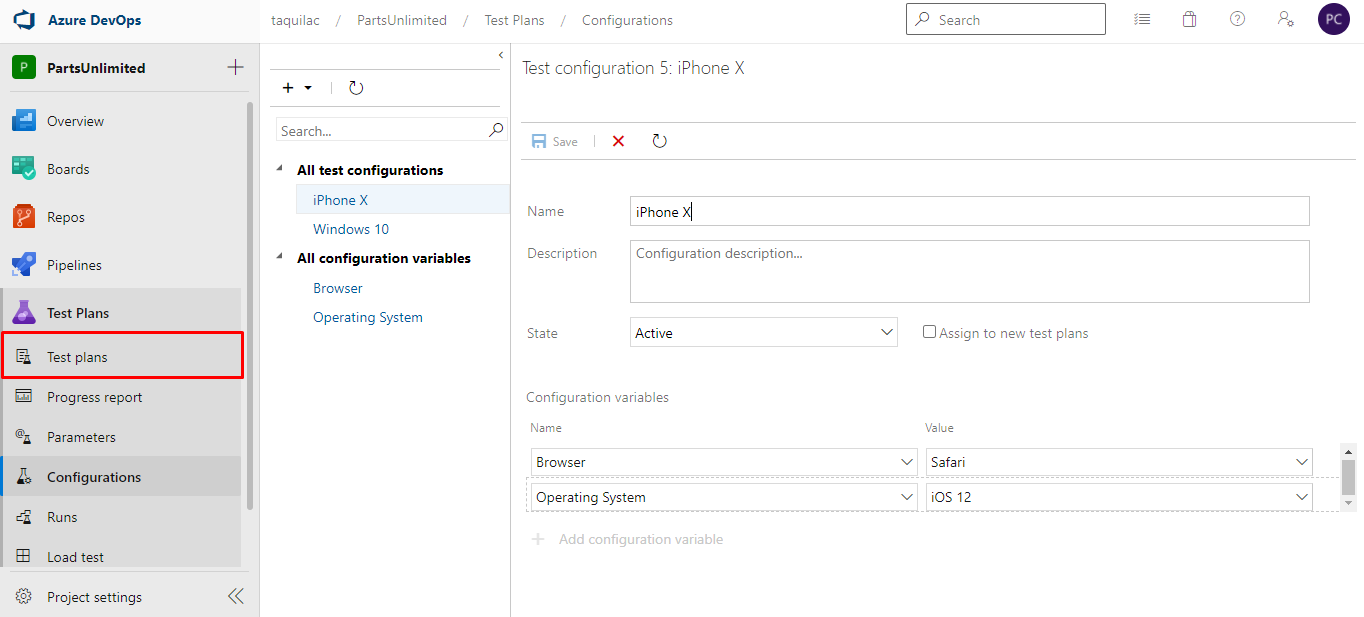
\includegraphics[width=15cm]{./Imagenes/27} 
\end{center}

17. Haga clic en el menú desplegable junto al conjunto de pruebas con el que hemos estado trabajando hasta ahora y seleccione Assing configurations to test suite\\

18. Marque la opción iPhone X y haga clic en Save.

\begin{center}
		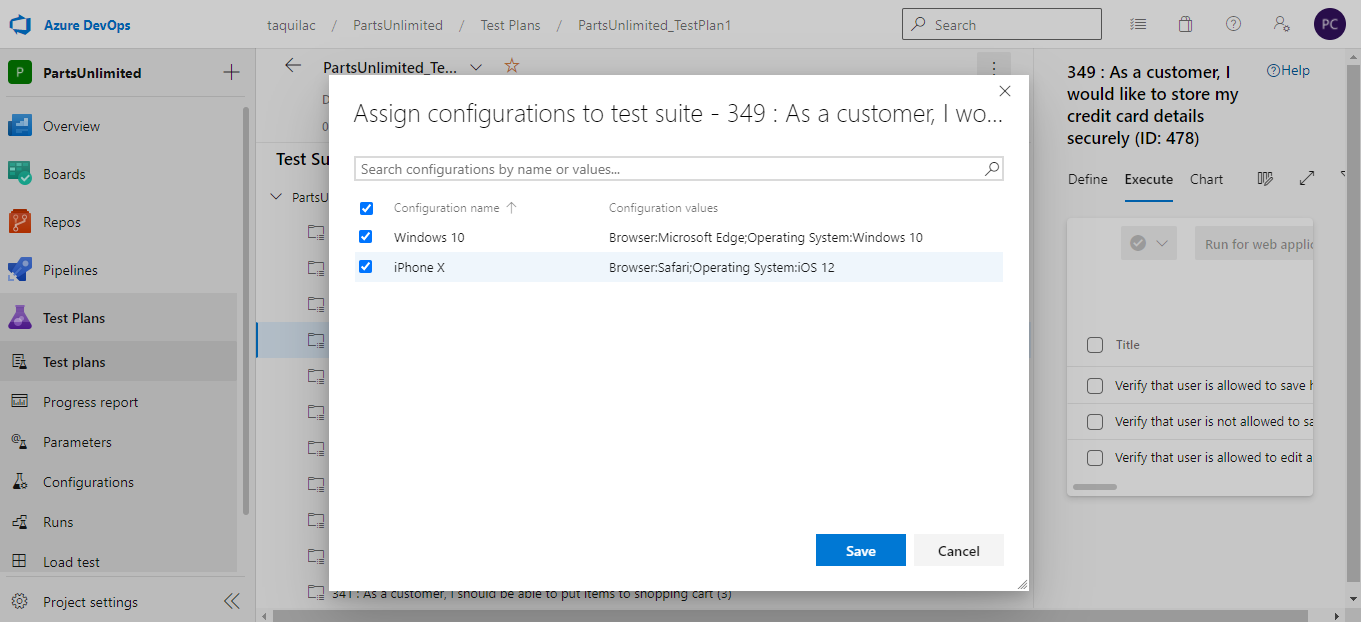
\includegraphics[width=15cm]{./Imagenes/28} 
\end{center}

19. Tenga en cuenta que cada caso de prueba se ha duplicado con una configuración adicional para iPhone X. Ahora cada entorno se puede probar y rastrear por separado.

\begin{center}
		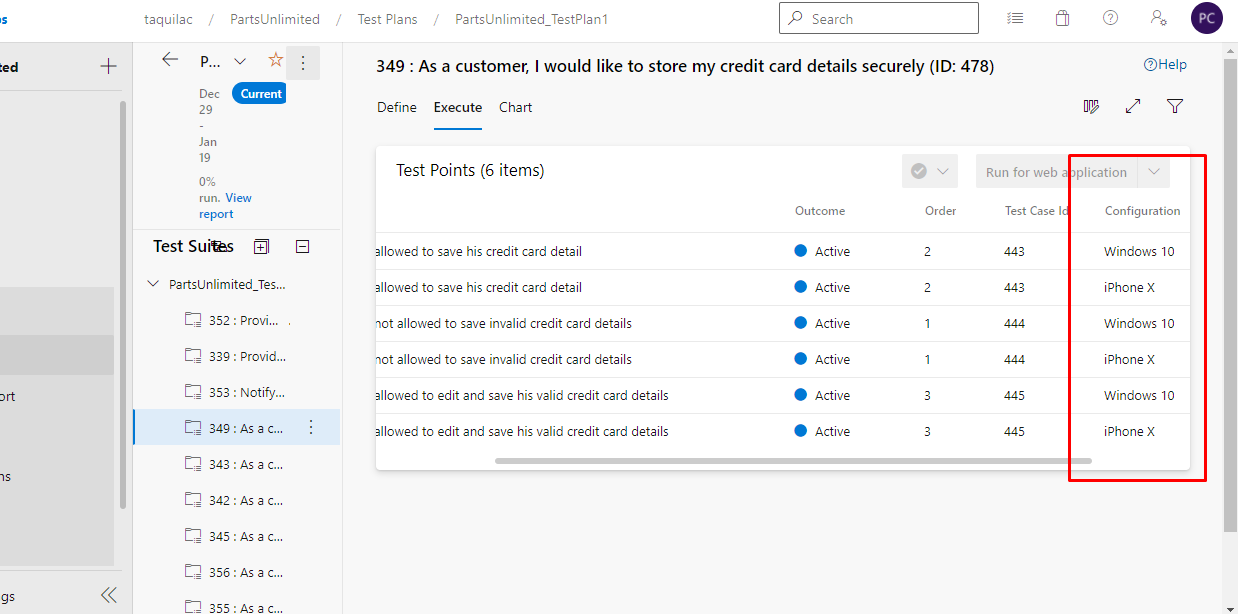
\includegraphics[width=15cm]{./Imagenes/29} 
\end{center}

\textbf{Tarea 3: Auditoria de Pruebas}\\

1. Expanda el menú desplegable junto al plan de prueba y seleccione New static suite. Un Static Suite de casos de prueba es un conjunto donde los casos se han asignado manualmente. También puede crear suites basado en requisitos comunes (requirement-based suite) o una consulta de casos de prueba y / o elementos de trabajo (query-based suite).

\begin{center}
		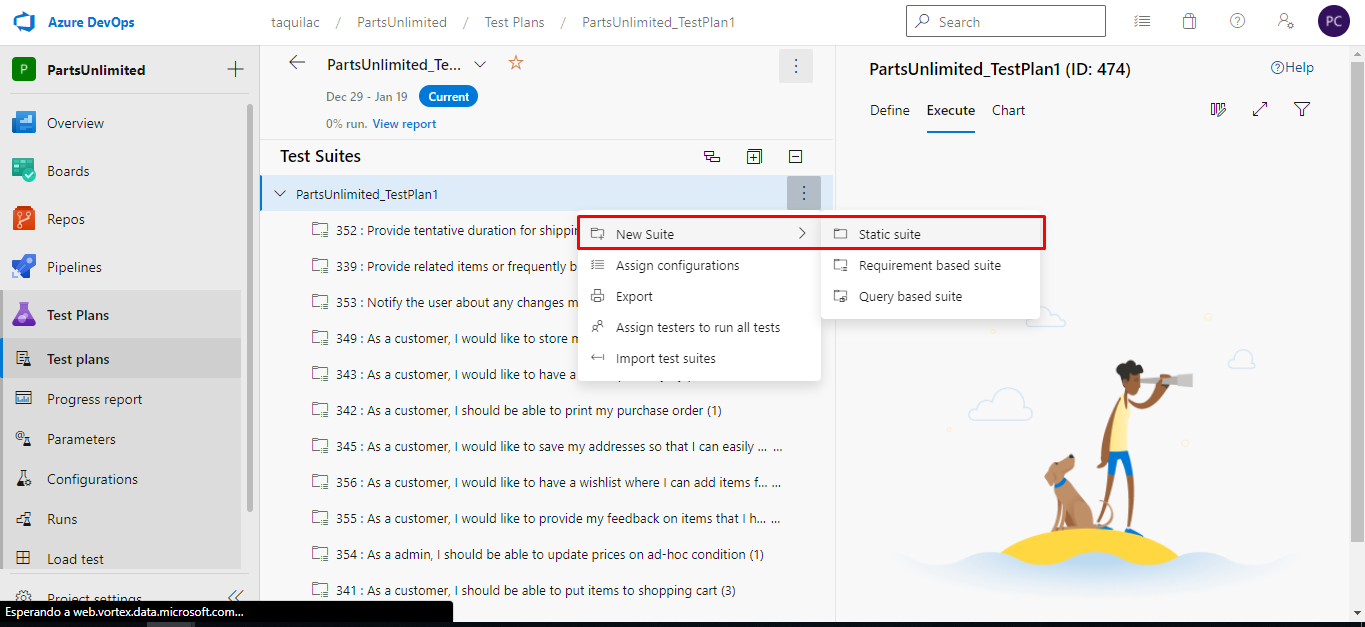
\includegraphics[width=15cm]{./Imagenes/30} 
\end{center}

2.Establezca el nombre de la nueva suite en "Shipping tests" . Todas estas pruebas se centrarán en la funcionalidad relacionada con el envío. Recuerde que puede compartir fácilmente casos de prueba entre suites, por lo que hay una redundancia mínima cuando hay muchas suites superpuestas.

\begin{center}
		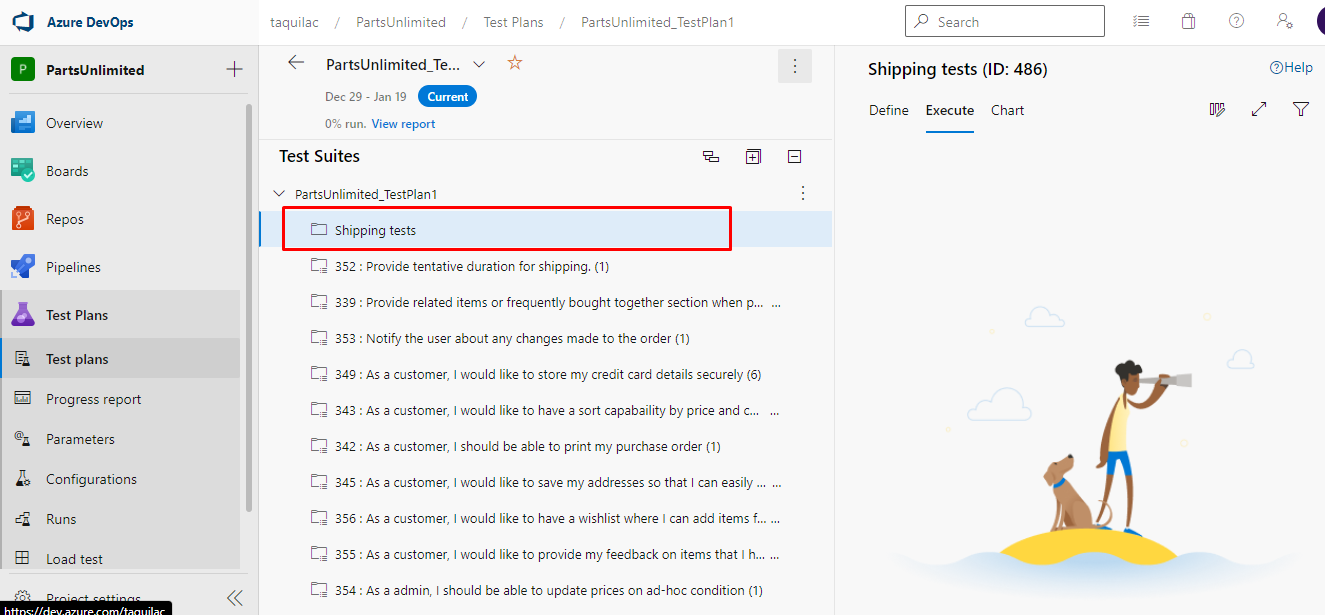
\includegraphics[width=15cm]{./Imagenes/31} 
\end{center}

3. Expanda el menú desplegable junto al paquete recién creado y seleccione New requirement-based suite.

\begin{center}
		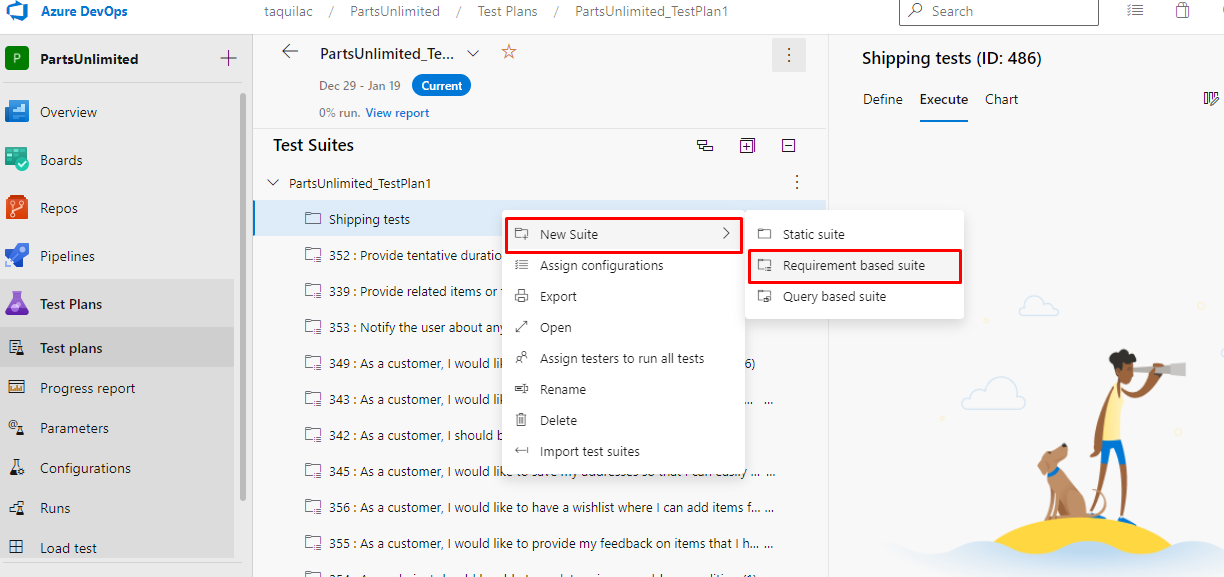
\includegraphics[width=15cm]{./Imagenes/32} 
\end{center}

4. Puede personalizar la consulta utilizada para especificar qué requisitos se recuperan, pero deje los valores predeterminados y haga clic en Run Query . Busque y seleccione los tres elementos de la cartera de productos relacionados con el envío. Haga clic en Create Suites para crear un conjunto de pruebas para cada uno.

\begin{center}
		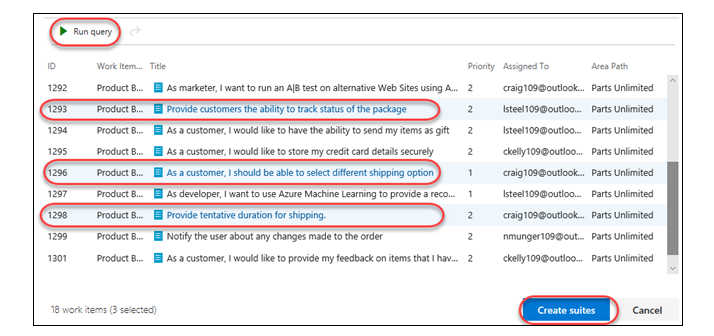
\includegraphics[width=15cm]{./Imagenes/40} 
\end{center}


5. Seleccione una de las suites recién creadas, como la asociada con el seguimiento del estado del paquete.

\begin{center}
		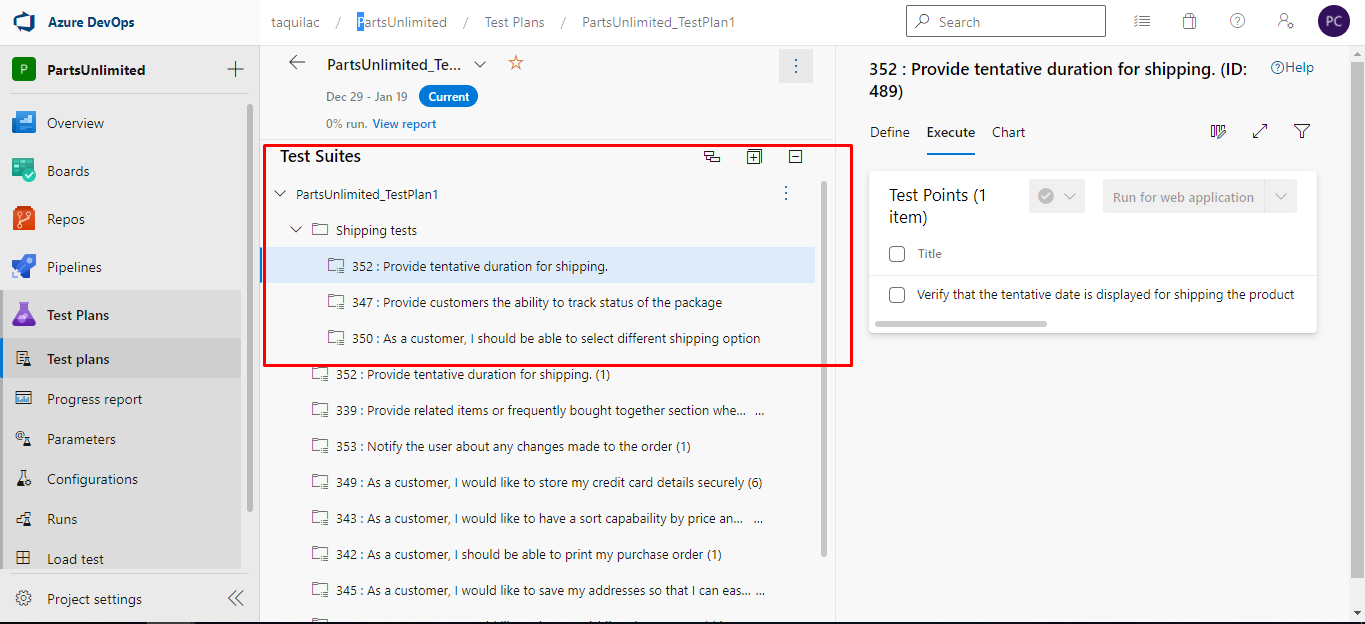
\includegraphics[width=15cm]{./Imagenes/33} 
\end{center}

6. Si bien puede crear casos de prueba uno a la vez, a veces es más fácil usar un diseño de cuadrícula para agregar rápidamente muchos casos de prueba. En el panel de casos de prueba, seleccione New | New test case using grid.

\begin{center}
		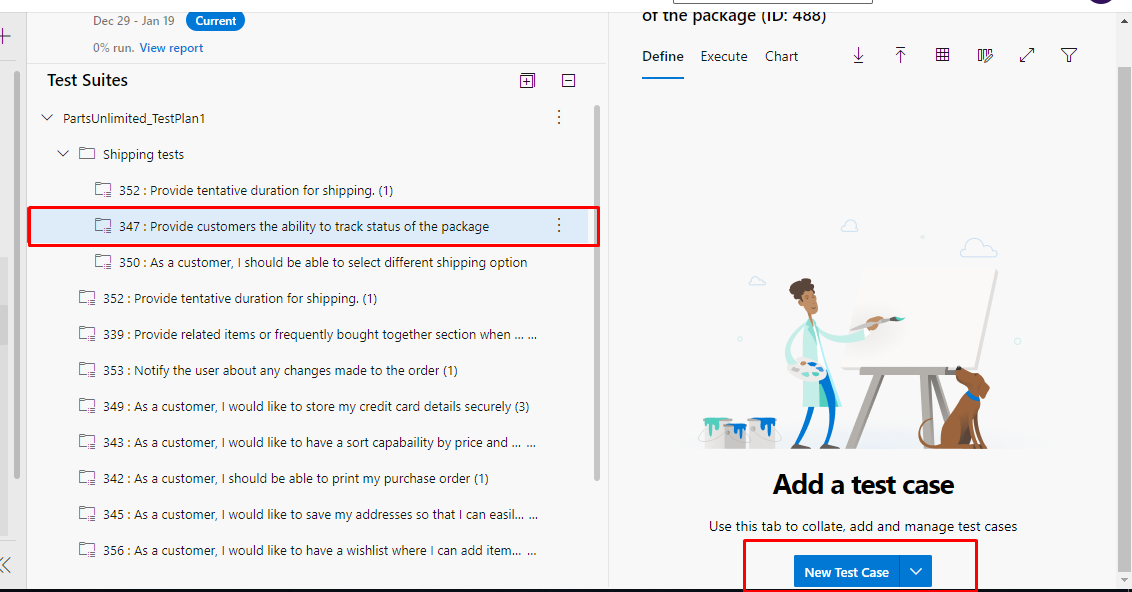
\includegraphics[width=15cm]{./Imagenes/34} 
\end{center}

7. Ingrese algunos casos de prueba y haga clic en el botón Save all. El título será el título eventual del caso de prueba. Step Action será el primer paso (y posiblemente el único) de la prueba. Si ese paso tiene un resultado esperado, puede especificarlo como Step Expected Result.

\begin{center}
		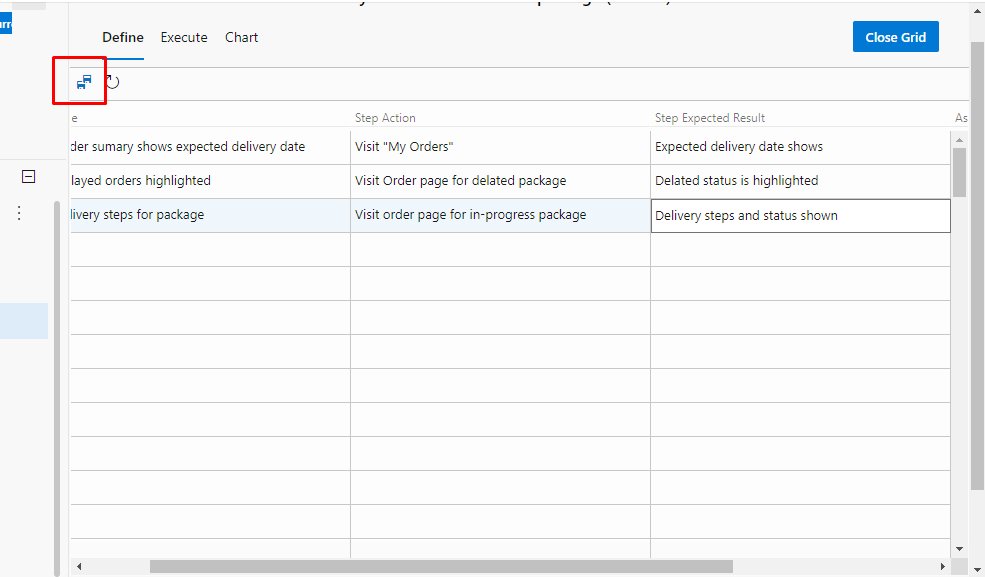
\includegraphics[width=15cm]{./Imagenes/35} 
\end{center}

8. Opcionalmente, puede continuar agregando y editando elementos de trabajo en la vista de cuadrícula. Cuando esté satisfecho, vuelva a la vista de lista haciendo clic en el botón Ver: Cuadrícula .

\begin{center}
		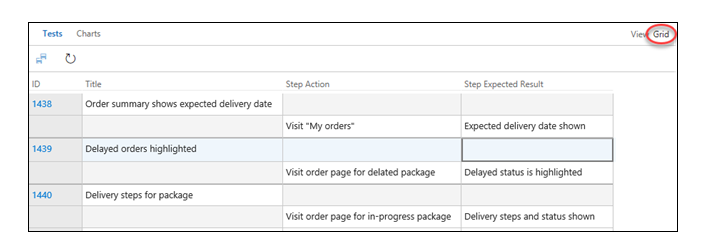
\includegraphics[width=15cm]{./Imagenes/39} 
\end{center}

9. La vista de lista muestra los mismos datos, pero en una vista diferente.

\begin{center}
		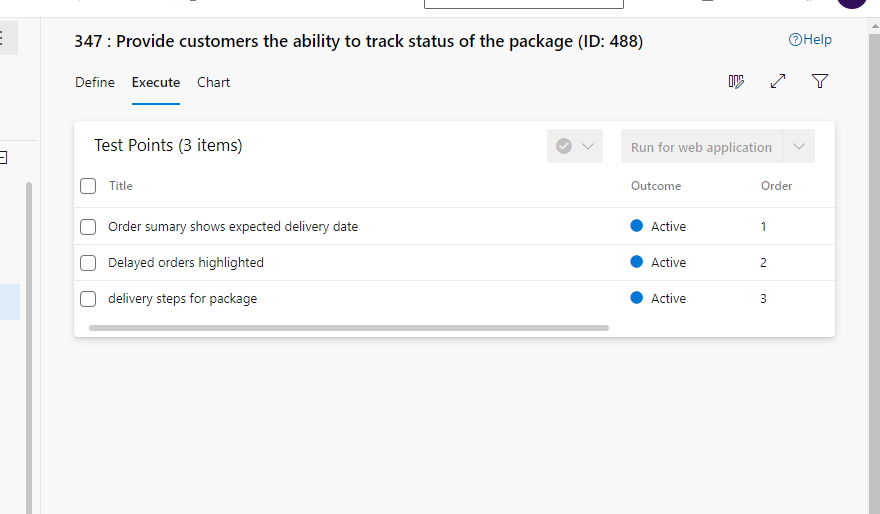
\includegraphics[width=15cm]{./Imagenes/36} 
\end{center}

10. Otra opción para crear conjuntos es mediante la consulta de elementos de trabajo. Expanda el menú desplegable junto al  Shipping tests de envío y seleccione un new query-based suite.

\begin{center}
		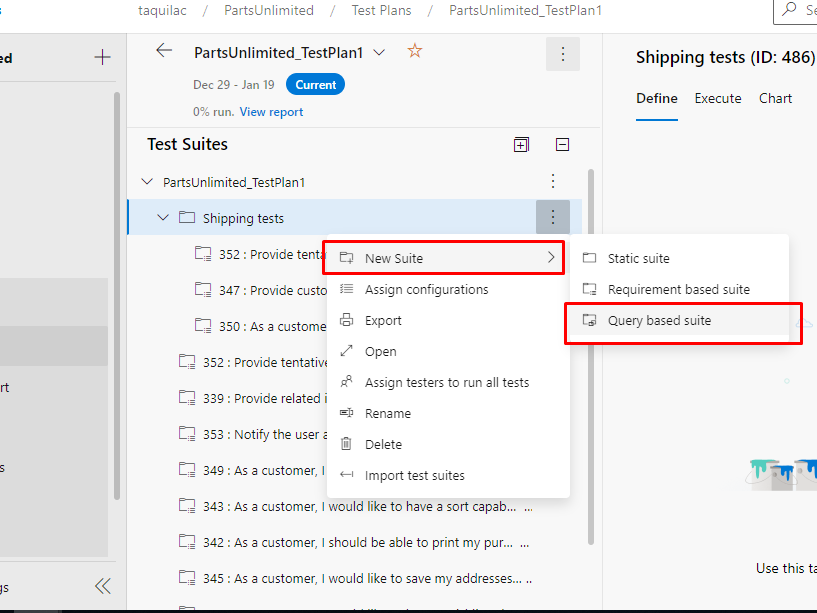
\includegraphics[width=15cm]{./Imagenes/37} 
\end{center}

11. Supongamos que desea crear un conjunto de pruebas a partir de casos de prueba relacionados con el envío en el proyecto. Cambie el Work Item Type a Microsoft.TestCaseCategory para buscar casos de prueba y haga clic en Run query. Ahora tiene una lista de casos de prueba que puede seleccionar para crear conjuntos, si lo desea.

\begin{center}
		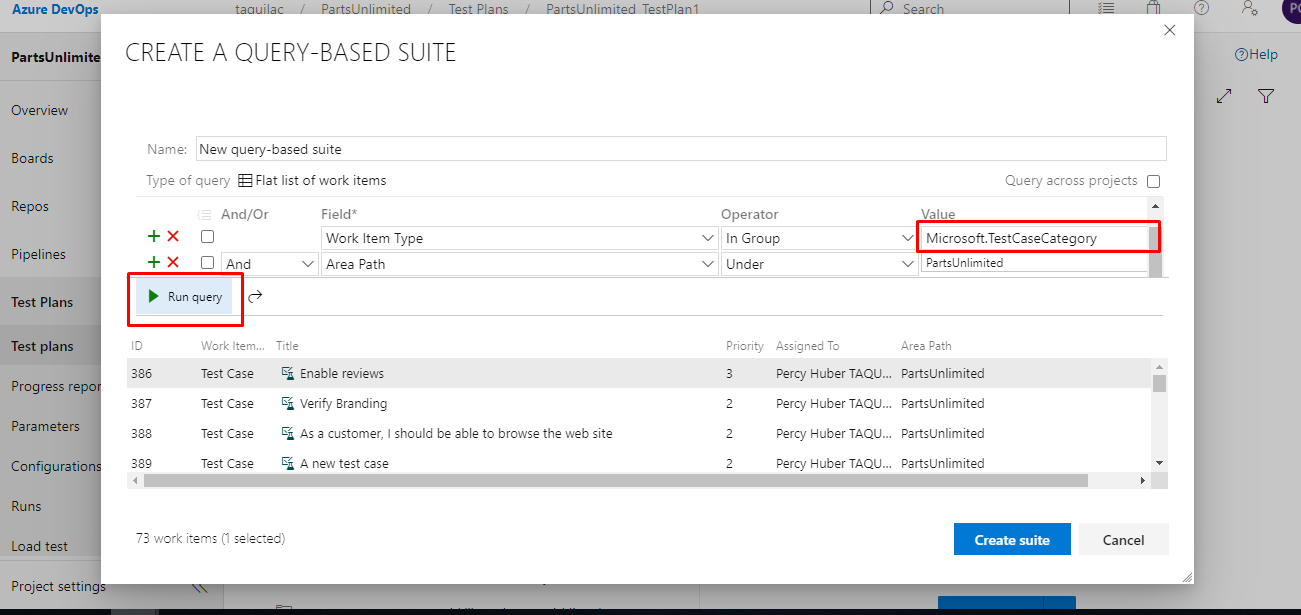
\includegraphics[width=15cm]{./Imagenes/38} 
\end{center}

12. Presione Esc para cerrar el diálogo.


\end{document}

